\ifx\wholebook\relax \else

\documentclass[UTF8]{article}

\usepackage[cn]{../prelude}

\setcounter{page}{1}

\begin{document}

% ================================================================
%                 Digit lock
% ================================================================

\title{锁车趣题}

\author{刘新宇
\thanks{{\bfseries 刘新宇} \newline
  Email: liuxinyu95@gmail.com \newline}
  }

\maketitle
\fi

\markboth{锁车趣题}{Unplugged}

\section{共享自行车}

在我撰写这一章节的时候,共享自行车正在流行。一些公司在城市的大街小巷投放一些自行车。如果一个人要使用,他需要支付一定的押金,然后就可以打开车锁骑走,共享自行车公司按照使用时间收费。到达目的地后,从押金中扣除使用费就可以了。

为了实现在任何时间、地点,都能够租、还车,自行车公司通过使用当时已经普及的智能手机,来实现自行车的租用、计时、收费。一个典型的场景大致如下:

\begin{enumerate}
\item 一个行人$p$在路边看到一辆上锁的共享自行车,这辆自行车上有一个唯一的编号$x$,他通过自己的手机联系自行车公司,告知他要使用这辆自行车;
\item 自行车公司收到这一行人$p$的请求,向他收取使用自行车$x$的押金;
\item 行人通过自己的智能手机向自行车公司支付押金;
\item 自行车公司收到押金后,通过某种方式打开自行车$x$的车锁;
\item 行人将自行车骑到某地点后,将自行车停好,并通过手机告知自行车公司他要还车;
\item 自行车公司收到请求后,根据自行车$x$的使用时间,从押金中扣除费用,将押金退还行人$p$,同时通过某种方式将自行车$x$锁好。
\end{enumerate}

这一使用方式中有一个环节非常关键:就是锁车。如果在退还押金后,没有将车锁上,此后的所有行人就可以“免费”使用这辆车了。为此,一些自行车公司制造了复杂的智能电子车锁。车锁能够和自行车公司通讯。这样自行车公司就能“遥控”打开和锁上自行车。还有的自行车公司,使用便宜的数字转盘密码锁,见图\ref{fig:normal-lock}。由于没有能够解决锁车问题,不得不派出工作人员,到大街小巷检查,看到没锁的自行车就锁上。甚至出现了有人在互联网上共享单车编号和密码对应表的情况。这样不想出钱的人,就可以通过自行车编号,查到密码,从而“免费”骑车。

\begin{figure}[htbp]
  \centering
  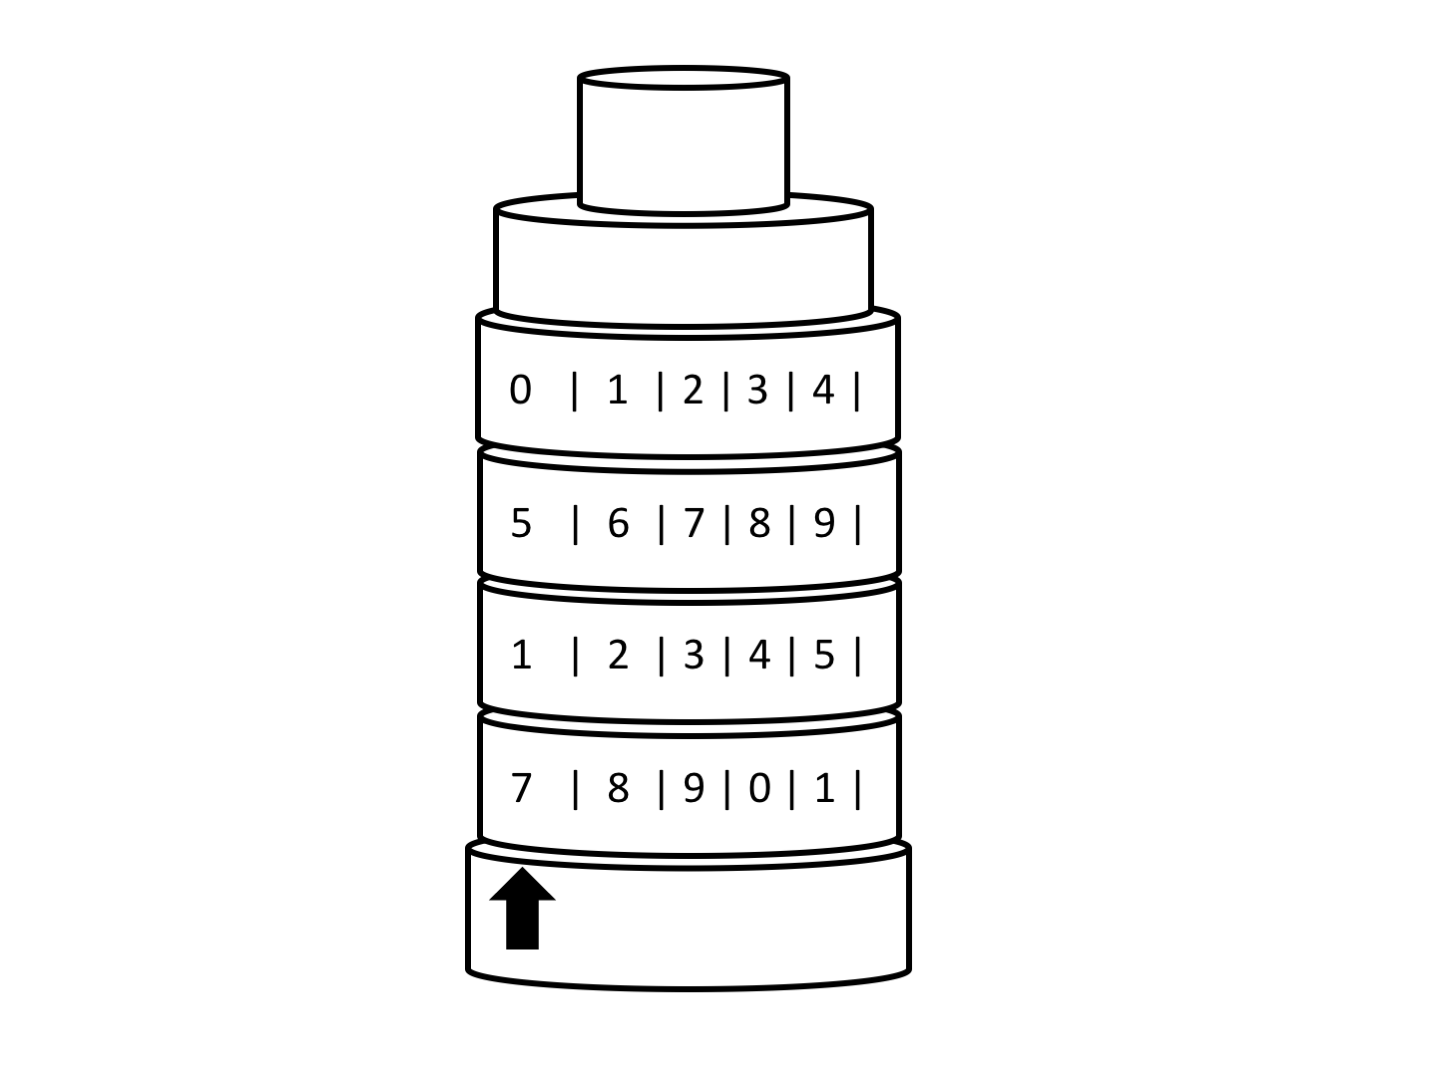
\includegraphics[scale=0.2]{img/normal-lock.eps}
  \caption{常见的数字转盘密码锁。每个转盘上按照顺序为0, 1, ..., 9共10个数字。图中4个转盘使得密码为0000到9999中的一个,共支持10000个密码。转动转盘,是的黑色箭头一行的数字为密码即可开锁。开锁后转盘被卡住不能转动。}
  \label{fig:normal-lock}
\end{figure}


有没有一种巧妙的方式,既不用使用电子设备,又能够解决锁车问题呢?

\section{巧解锁车趣题}

解决锁车趣题的关键在于,我们需要通过某种方式,确认自行车已经上锁后,才停止计费。怎样才能进行这种确认呢?以图\ref{fig:normal-lock}中的密码锁为例,开锁时,乘客将自行车的编号$x$通过手机发给自行车公司,自行车公司开始计费后,将$x$对应的4位密码发到行人的手机上,例如7150,行人转动密码盘,使得黑色箭头对准7150,就可以开锁了。当乘客停好车,通过手机联系自行车公司要求停止计费时,自行车公司可以发给乘客一个随机4位数字$y$,例如3194,要求乘客将密码盘拨到这个数字才停止计费。由于密码盘只有在上锁后才能转动。因此这个问题就转换为了:如何保证乘客将密码盘转动到某一指定数字上才停止计费的问题。

但这个新问题丝毫不比老问题简单。如果能够让密码锁有某种“计算”功能,当乘客收到自行车公司发来的$y$,他必须锁车后,转动密码盘得到另一数字$z=f(y)$。然后行人将$z$发回给自行车公司验证,验证成功后才停止计费。这样就能解决锁车难题了。

接下来就要想出如何实现上述的“计算”功能。其中一种方法就是让每个密码盘上的数字顺序不是简单的从0、1增加到9,而是某种随机的顺序。如图\ref{fig:random-lock}(b)所示。

\begin{figure}[htbp]
  \centering
  \subfloat[普通锁的密码盘都是从0到9的顺序。]{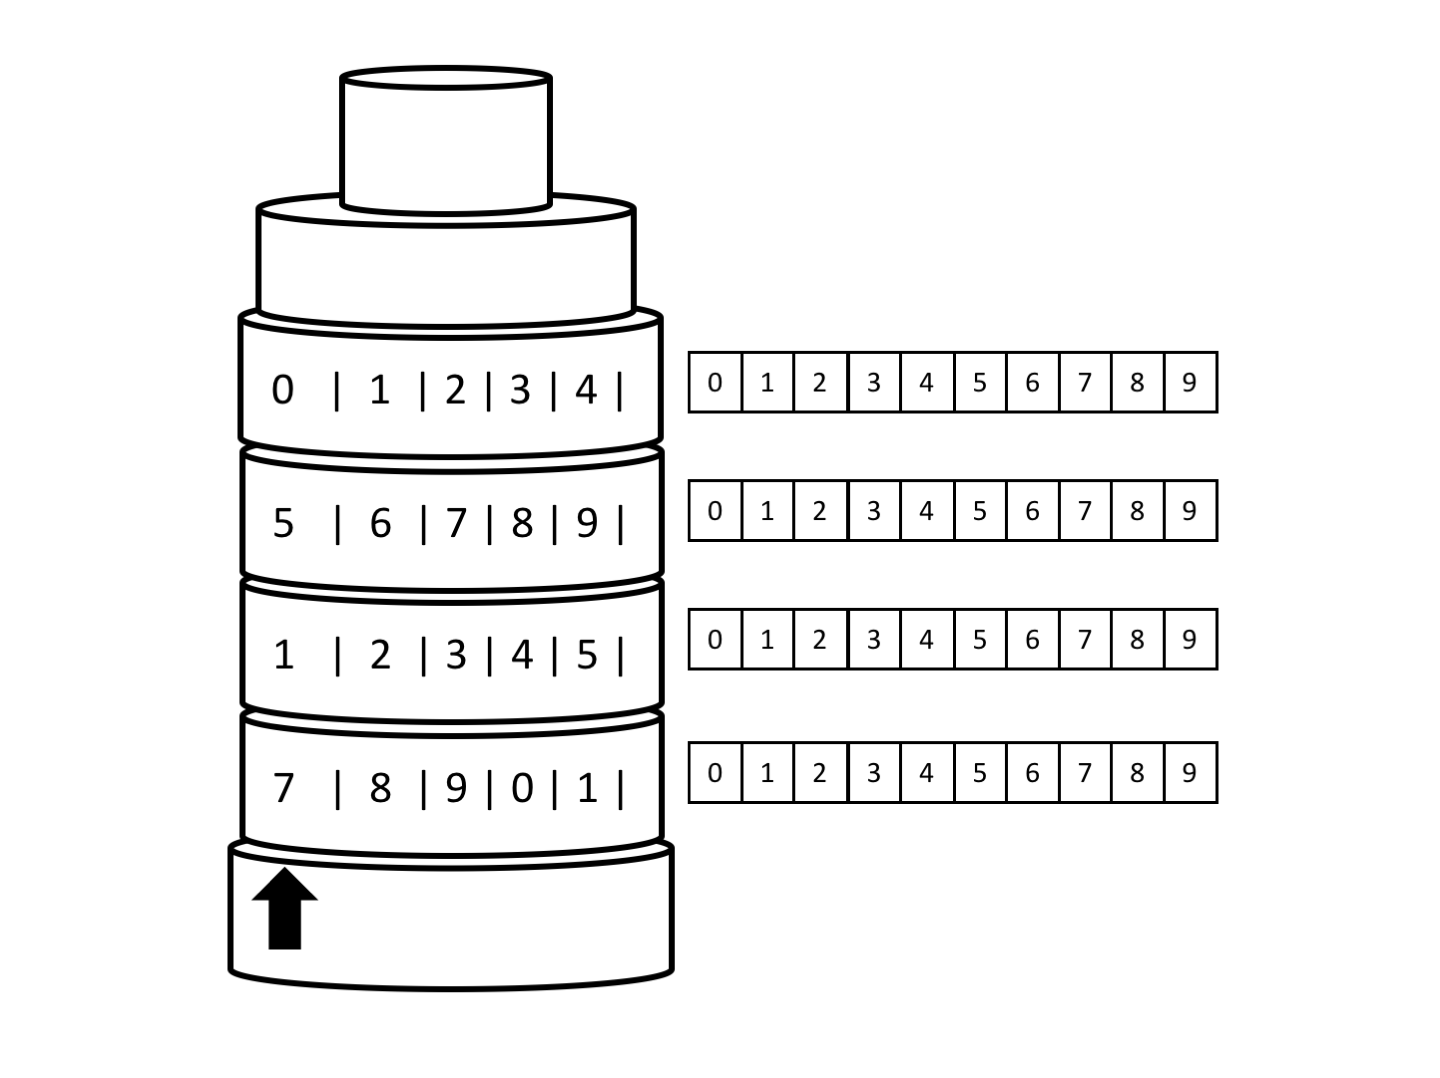
\includegraphics[scale=0.2]{img/normal-digits-order.eps}} \\
  \subfloat[密码盘上的10个数字顺序是随机的。]{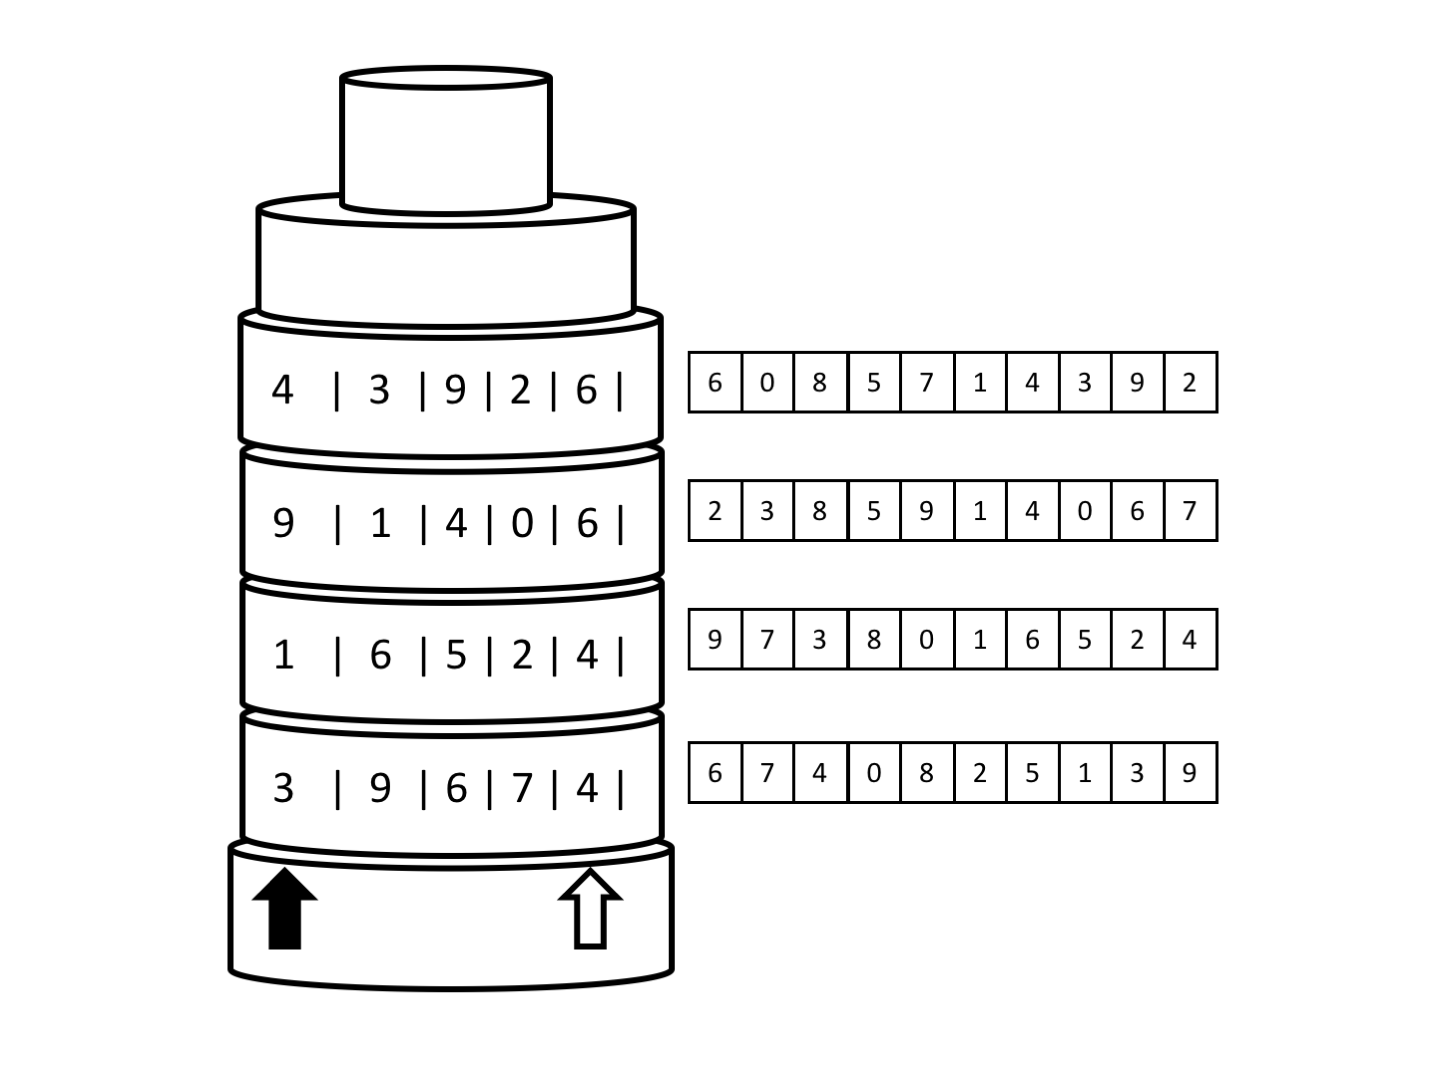
\includegraphics[scale=0.2]{img/random-digits-order.eps}}
  \caption{四个密码盘上的数字的顺序都是随机印上去的,同时增加一个白色箭头。}
  \label{fig:random-lock}
\end{figure}

每个密码盘上的10个数字顺序是随机的,自行车公司事先知道每辆自行车上的密码盘数字顺序。当行人到达目的地停车时,他通过手机告诉自行车公司申请停止计费。自行车公司生成一个4位随机数,例如3194发到行人的手机上,并要求行人拨动车锁密码盘,使得黑色箭头对准3194,然后将白色箭头对准的数字发回。由于行人必须锁车后才能拨动密码盘,所以他只能先锁好车。拨到3194,然后将白色箭头对准的数字,按照图中的例子,也就是4466发回给自行车公司。由于自行车公司事先知道编号为$x$的自行车锁的密码盘顺序,所以可以核对4466是否正确。如果正确就通知行人停止计费。这一过程如图\ref{fig:lock-diagram}所示。

\begin{figure}[htbp]
  \centering
  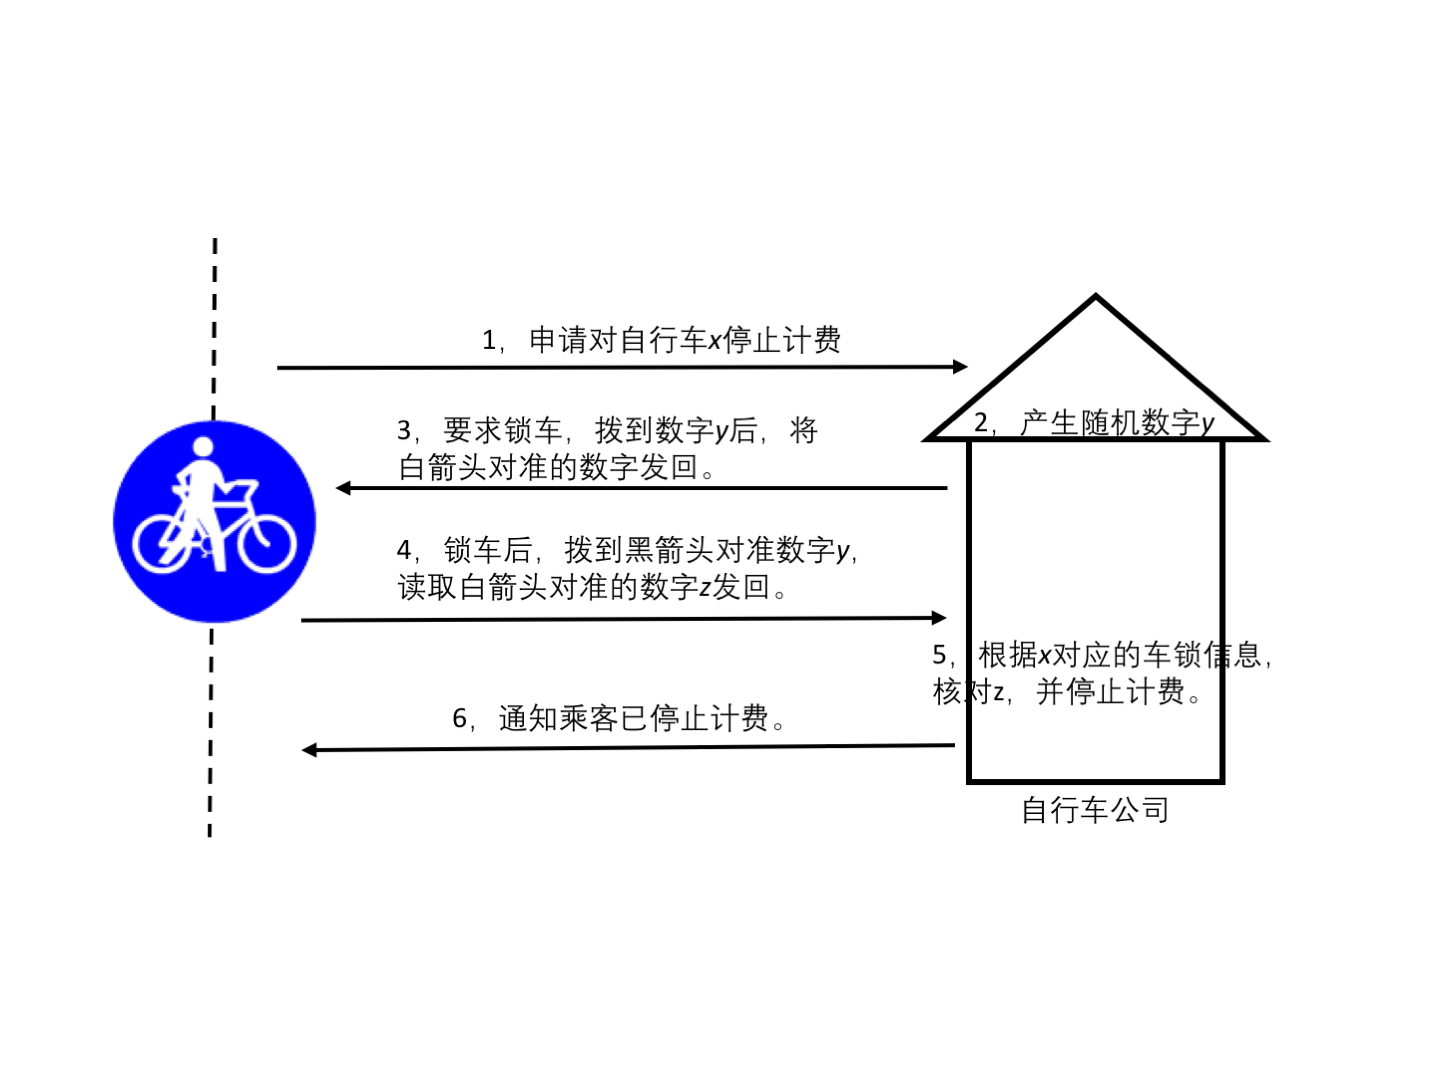
\includegraphics[scale=0.2]{img/diagram.eps}
  \caption{验证锁车、并停止计费的过程。}
  \label{fig:lock-diagram}
\end{figure}

这一过程对于大多数正常使用自行车的人都有效。由于密码盘的随机性,行人收到自行车公司要求拨到的数字后,不锁车而直接猜测出白色箭头对应的数字的难度较大。但是这一解法仍然存在一个严重的漏洞。

\section{亡羊补牢}
由于行人一旦开锁用车,他就知道自行车的密码了。尽管在最后还车的环节,我们迫使他锁车并旋转密码锁到指定的位置以结束计费,但是行人一旦确认计费已经停止,他可以再次用记住的密码打开车锁,然后离开。

为了解决这一漏洞,自行车公司可以设置“锁车举报奖励”。即任何行人,如果发现某辆车没有锁,他可以申请获得举报奖励。申请方法如下:

\begin{enumerate}
\item 行人使用手机,通知自行车公司,他发现自行车$x$没有锁。申请获得奖励;
\item 自行车公司收到请求后,要求行人发来自行车锁上黑色箭头对准的数字(即开锁密码)进行验证;
\item 验证后,自行车公司产生一随机数字$y$,要求行人锁车,并将密码锁拨到数字$y$,然后将白色箭头所对准的数字发回;
\item 行人锁车后,转动密码锁,使得黑色箭头对准$y$,然后读出白色箭头对准的数字$z$,发回给自行车公司;
\item 自行车公司收到$z$后,根据自行车$x$的密码盘信息,验证$z$。如正确,就把奖励金发给行人;
\end{enumerate}

简单来说,锁车举报验证的过程和上述锁车过程的解法类似。自行车公司迫使行人锁车后才发放奖励。为了避免在得知他人的用车密码后,反复骗取锁车奖励金的行为,自行车公司还需要监控是否某一辆自行车被多次领取奖励金。

\begin{Exercise}
为了惩罚锁车后又故意打开自行车的行为,自行车公司决定从最后一次使用该自行车的顾客的押金内扣除费用,以奖励举报。请问这样做合理么?会出现什么潜在的问题?
\end{Exercise}

\ifx\wholebook\relax \else
%% \begin{thebibliography}{99}

%% \bibitem{fp-pearls}
%% Richard Bird. ``Pearls of functional algorithm design''. Cambridge University Press; 1 edition (November 1, 2010). ISBN-10: 0521513383

%% \bibitem{Bentley}
%% Jon Bentley. ``Programming Pearls(2nd Edition)''. Addison-Wesley Professional; 2 edition (October 7, 1999). ISBN-13: 978-0201657883 (中文版:《编程珠玑》)

%% \bibitem{okasaki-book}
%% Chris Okasaki. ``Purely Functional Data Structures''. Cambridge university press, (July 1, 1999), ISBN-13: 978-0521663502

%% \bibitem{CLRS}
%% Thomas H. Cormen, Charles E. Leiserson, Ronald L. Rivest and Clifford Stein. ``Introduction to Algorithms, Second Edition''. The MIT Press, 2001. ISBN: 0262032937. (中文版:《算法导论》)

%% \end{thebibliography}

\expandafter\enddocument
%\end{document}

\fi
